\lecture{4}{7/2}
\begin{definition}[3D scene]
    A \textbf{3D scene} is a space defined by a 3D coordinate system.
\end{definition}

It comprises of \emph{3D objects}.
Objects have \emph{local coordinates} relative to an \emph{origin}.
We also have a single global set of coordinates called \emph{world coordinates}.

Local coordinates reduce complications in scene construction.

\begin{definition}[View transform]
    A \textbf{view transform} will transform world coordinates to the
    view origin, where our camera is located.
\end{definition}

This transform allows us to specify how 2D images of a 3D scene are rendered.

We also have a \textbf{projection transform}.

\begin{figure}[]
    \centering
    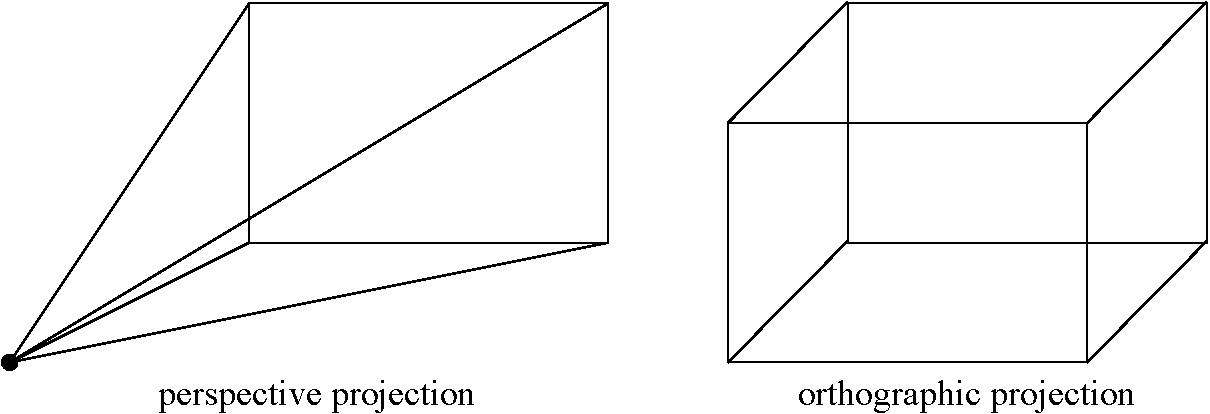
\includegraphics[width=0.8\linewidth]{images/perspective-orthographic-projection.pdf}
    \caption{A diagram illustrating both perspective projection and
             orthographic projection.
    }%
    \label{fig:perspective-orthographic-projection}
\end{figure}

\begin{definition}[View frustrum]
    The \textbf{view frustrum} is the region of space in a modelled world
    that may appear on the screen;
    it is the field of view of a perspective virtual camera system.
\end{definition}

\begin{figure}[]
    \centering
    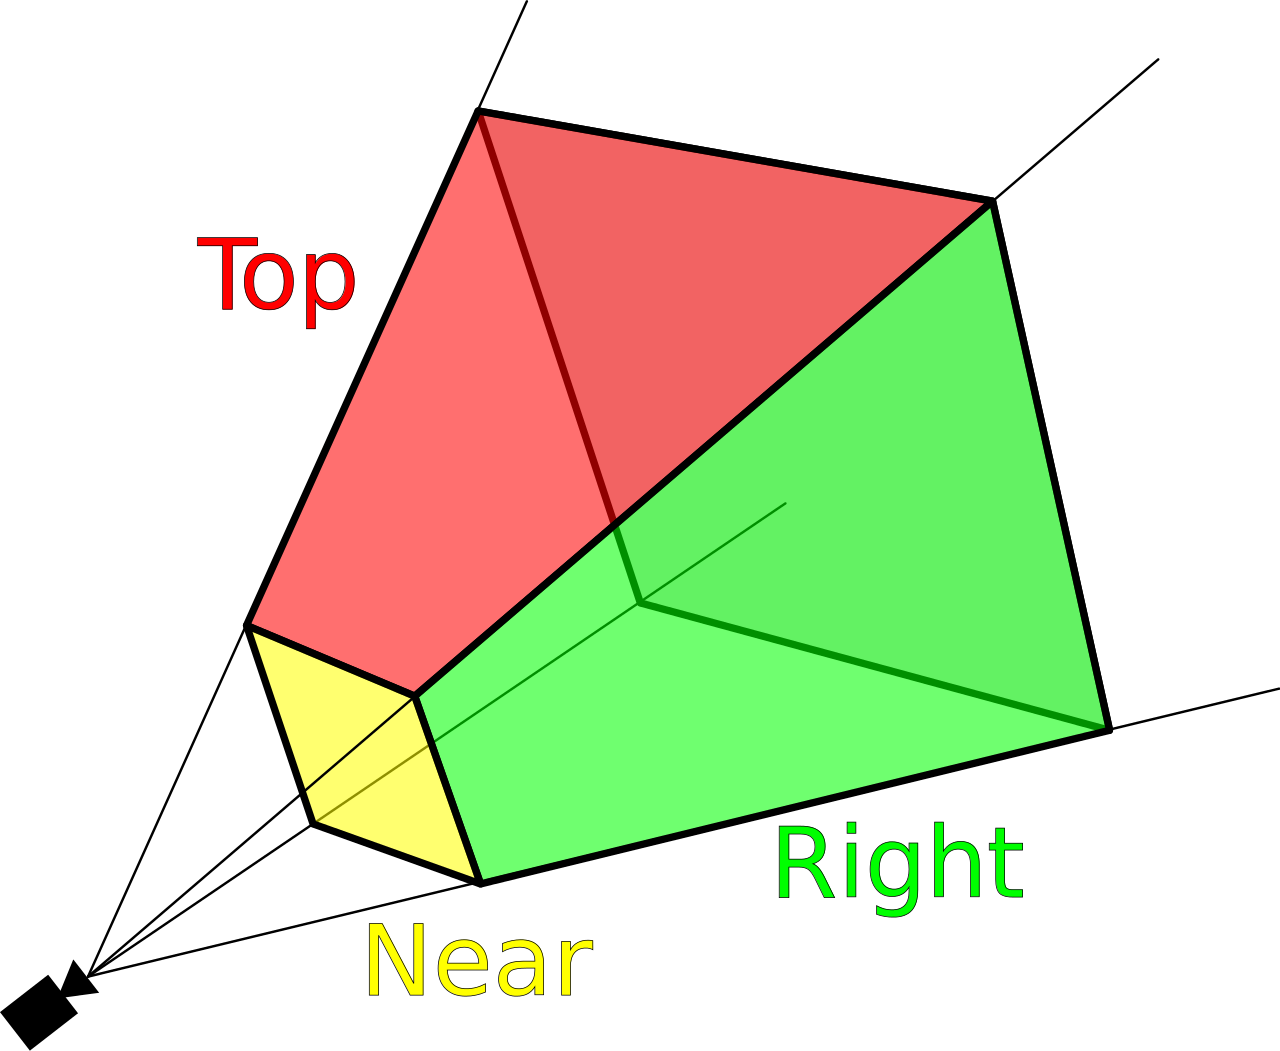
\includegraphics[width=0.8\linewidth]{images/view-frustrum.png}
    \caption{A view frustrum.}%
    \label{fig:view-frustrum}
\end{figure}

If the near plane is the same dimesnion of the far plane, we get an 
\emph{orthographic projection}. 
Otherwise, it is a perspective projection.
